\subsection{Efficient Inference and Long-Video Processing}
\label{sec:efficiency}
\subsubsection{One-Step and Few-Step Restoration}
For a latent restoration pipeline, an approximate inference decomposition is
\begin{equation}
\begin{split}
\mathcal C_{\mathrm{total}}={}&\mathcal C_{\mathrm{encode}}
+\sum_{i=1}^{N_{\mathrm{FE}}}\mathcal C_{\mathrm{denoise},i}
+\mathcal C_{\mathrm{decode}}\\
&+\mathcal C_{\mathrm{aux}}+\mathcal C_{\mathrm{stitch}}.
\end{split}
\label{eq:cost}
\end{equation}
$N_{\mathrm{FE}}$ counts actual denoiser evaluations, including extra calls used by guidance when applicable, and $\mathcal C_{\mathrm{denoise},i}$ allows different costs for base and draft networks. The auxiliary term covers predictors, flow estimation, reference processing, and additional optimization outside these calls; the remaining terms cover autoencoding and spatial/temporal assembly. This decomposition explains why reducing sampling steps does not translate directly into an equal end-to-end speedup: encoding, decoding, and condition processing can dominate once repeated denoising becomes cheap. Parallel execution further affects the relationship between computation and latency.

One-step methods attack the repeated-denoising term. DOVE uses latent-pixel training, DLoRAL separates consistency and detail adaptation, UltraVSR combines one-step reconstruction with temporal mechanisms, and OS-DiffVSR uses multi-frame fusion and adjacent-frame adversarial training~\cite{dove,dloral,ultra,osdiff}. SeedVR2 uses distillation and adversarial post-training for generic restoration~\cite{seedvr2}. Their training objectives absorb detail synthesis, observation fidelity, and temporal regularity into a small number of evaluations, shifting computational effort from inference to adaptation or distillation.

Distillation must retain temporal behavior as well as single-frame realism. DUO-VSR progressively compresses a multistep teacher, then combines distribution matching with adversarial features from real and fake score models before preference-guided refinement~\cite{duovsr}. Its teacher is based on an internal 1.3B text-to-video model. AdcVSR transfers a DOVE teacher into a pruned SD2.1-based student with lightweight one-dimensional temporal convolutions~\cite{adcvsr}. Its pixel and feature discriminators each separate detail assessment from consistency assessment, making the potential conflict between these objectives explicit in the supervision. InstaVSR also uses a pruned image-diffusion backbone, but combines latent- and pixel-space adversarial learning with recurrent training and flow-guided temporal regularization~\cite{instavsr}. The latter predicts an output frame from five input frames, combining local multi-frame evidence with recurrent temporal supervision. These methods support a useful distinction between inheriting temporal structure from a video teacher, adding temporal computation to the student, and imposing temporal supervision during training.

Intermediate designs preserve selective refinement instead of forcing all restoration into one identical model evaluation. PS-SR assigns global reconstruction to one expensive base-model prediction and high-frequency refinement to a pruned draft model~\cite{pssr}. Its default four-stage configuration comprises one base evaluation and three draft evaluations, and the frequency-restricted update helps retain the low-frequency anchor. The term pseudo-single-step therefore describes an asymmetric computational budget rather than a single total function evaluation. SATB-VR takes a different approach: an auxiliary predictor initializes a higher-SNR state, SNR-aware trajectory blending trains the denoiser to tolerate prediction error, and denoiser-driven feature consistency improves the predictor~\cite{satbvr}. Its flexible few-step schedule preserves opportunities for correcting the initial estimate. These approaches retain selective correction after initialization, trading a small amount of additional computation for greater flexibility than a direct prediction. Table~\ref{tab:efficiency} summarizes complementary approaches to reducing computation. The number of generative updates, the cost of each update, and the amount of temporal buffering define different aspects of efficiency.

\begin{table*}[t]
\caption{Representative acceleration strategies. Sampling counts refer to the cited configurations; auxiliary prediction, encoding, decoding, and temporal buffering remain part of the complete system.}
\label{tab:efficiency}\centering\footnotesize
\begin{tabularx}{\textwidth}{@{}p{0.15\textwidth}p{0.16\textwidth}YY@{}}\toprule
Method & Generative updates & Principal cost reduction & Remaining computation / context \\\midrule
DOVE~\cite{dove} & One & One-step adaptation with latent-then-pixel training & Video DiT and autoencoder; joint clip context \\
TurboVSR~\cite{turbo} & Four-step setting & Highly compressed tokens and nonuniform shortcut learning & Spatiotemporal autoencoder and factorized conditioning \\
PS-SR~\cite{pssr} & One base + three draft & Expensive structure prediction followed by lightweight refinement & Four network evaluations of unequal cost \\
FastVSR~\cite{fastvsr} & One & Asymmetric encoder/decoder and compressed denoising grid & Spatial expansion and detail reconstruction in the decoder \\
AdcVSR~\cite{adcvsr} & One & Pruned image-prior student with lightweight temporal layers & Multi-frame processing; distillation from DOVE \\
OASIS~\cite{oasis} & One & Specialized attention and replacement of the VAE encoder & Video denoiser and decoder; learned input projection \\
InstantViR~\cite{instantvir} & Feedforward solver & Amortized inference, cached state and LeanVAE & Bidirectional context within each buffered block \\
SATB-VR~\cite{satbvr} & One--ten-step schedules & High-SNR initialization and trajectory blending & Auxiliary predictor plus selected denoising updates \\\bottomrule
\end{tabularx}
\end{table*}

\subsubsection{Representation and Network Compression}
Reducing denoiser evaluations is only one route to lower latency. TurboVSR reduces the number of tokens through an LTX autoencoder with $32\times32\times8$ compression, factorizes first-frame and remaining-frame conditioning, and converts the denoiser to a nonuniform shortcut model with a four-step operating point~\cite{turbo}. FastVSR instead changes the autoencoder interface: an asymmetric $f8$ encoder and $f16$ decoder permit a smaller denoising representation, with spatial expansion deferred to decoding and lower-bound-guided training used to stabilize the decoder~\cite{fastvsr}. OASIS removes further computation through attention-head specialization, replaces the VAE encoder with pixel unshuffle and linear projection, and progressively trains on temporally consistent and then inconsistent degradations~\cite{oasis}. Together, these designs show why step count is an incomplete cost measure. Token resolution, temporal compression, attention structure, and autoencoding jointly determine the end-to-end computational cost. High compression may reduce the computational burden while changing the evidence available for fine detail and motion reconstruction.

\subsubsection{Spatial Tiling and Temporal Windows}
At high resolution, memory may be dominated by latent features, attention activations, or decoding. Spatial tiling reduces peak memory but removes context and introduces stitching boundaries. PatchVSR and DC-VSR explicitly exchange information beyond isolated patches~\cite{patch,dcvsr}. Tile dimensions, overlap, and blending determine how much boundary context is retained. Global information from the full input can reduce semantic disagreement between tiles.

Temporal windows face a similar tradeoff. Overlapping clips provide local bidirectional context but repeat computation and may yield inconsistent boundary frames. Variable-size or shifted windows, as in SeedVR, address context management inside the model~\cite{seedvr}. External window blending can hide discontinuities without solving global identity drift. Boundary artifacts can consequently remain even when the interior of each clip is restored well.

\begin{figure*}[t]
\centering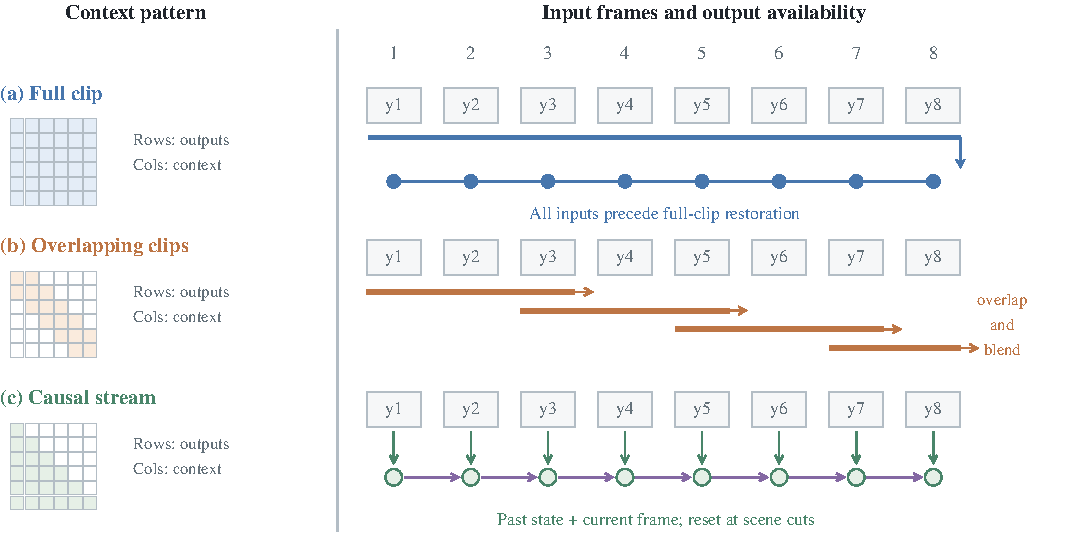
\includegraphics[width=\textwidth]{figures/deployment.pdf}
\caption{Temporal context in full-clip, overlapping-window, and causal inference. The matrices show allowed context interactions; the right-hand diagrams illustrate frame access and propagation. Full-clip processing uses future frames, overlapping windows reuse local context, and causal streaming carries state from past observations.}
\label{fig:deployment}
\end{figure*}

\subsubsection{Causality, Throughput, and Latency}
Figure~\ref{fig:deployment} distinguishes full-clip processing, overlapping windows, and causal streaming. Throughput measures sustained output rate; latency measures the delay experienced by an input frame or by the first output. A method can process a completed clip quickly while requiring the entire clip in advance. It can also have high steady-state throughput while buffering several future frames.

Stream-DiffVSR uses a four-step, frame-causal process with motion-aligned autoregressive guidance and temporal decoding~\cite{stream}. Its initialization descends from the StableVSR upscaler lineage. FlashVSR combines one-step inference, sparse attention, and a compact conditional decoder, while InfVSR uses causal transformer processing with a rolling cache~\cite{flash,infvsr}. Chunk-oriented streaming can introduce future-frame waiting within a chunk, so its look-ahead should not be equated with zero-latency framewise causality. SwiftVR extends the efficiency discussion to generic restoration with chunkwise processing and a restoration-aware autoencoder~\cite{swiftvr}.

An adequate timing report includes hardware, precision, input/output resolution, clip length, batch size, frame rate, number of warm-up iterations, peak memory, first-output latency, and steady-state throughput. It should state whether file decoding, transfer, flow, VAE execution, and output encoding are included. CPU offloading can make a method fit memory while substantially changing latency. Reporting only the fastest isolated network kernel does not describe deployed restoration.

\subsubsection{Long-Horizon Memory and Error Accumulation}
Long-video processing requires more than support for an arbitrary number of chunks. Persistent state can drift, propagate an incorrect detail, or lose an identity after occlusion. LiftVSR's cross-segment attention memory and InfVSR's rolling cache exemplify attempts to retain useful context~\cite{lift,infvsr}. Their design also motivates tests with long occlusions, return-to-scene events, shot changes, and objects leaving and entering the view.

A useful evaluation plots fidelity and temporal behavior as a function of elapsed video time, rather than only aggregating all frames. State resets should be logged, and the benchmark should contain both continuous shots and edited sequences. For interactive use, the system must also handle an input rate that exceeds its sustained processing capacity: queue growth, frame dropping, and adaptive quality control are part of the deployment problem. These system properties cannot be inferred from the label ``one-step.''
